\documentclass[11pt]{article}

%% compile with option -shell-escape if including .eps file.
%% $ pdflatex -shell-escape mydoc.tex

\usepackage{amsmath}
\usepackage{amssymb}
\usepackage{amsthm}
\usepackage{appendix}
\usepackage{multirow}
\usepackage[pdftex]{graphicx}
\usepackage{epstopdf}
\usepackage{listings}
\usepackage{url}
%% \usepackage[margin=2cm]{geometry}

\pdfpagewidth 8.5 in
\pdfpageheight 11 in

\setlength\topmargin{0in}
\setlength\headheight{0in}
\setlength\headsep{0in}
\setlength\textheight{9.0in}
\setlength\textwidth{6.5in}
\setlength\oddsidemargin{0in}
\setlength\evensidemargin{0in}
\setlength\parindent{0.25in}
\setlength\parskip{0.0cm}

\title{CSI 722: Uniform Grid Generation}
\author{Student: Andrew Kercher \\ Professor: R. L\"{o}hner}
\date{Fall 2011}

\begin{document}
\maketitle
%% \tableofcontents

%% \newcommand{\mycommand}[number of parameters]{definition of this command}
\newcommand{\be}[1]{\begin{#1}}
\newcommand{\eb}[1]{\end{#1}}
\newcommand{\beenum}[0]{\begin{enumerate}}
\newcommand{\ebenum}[0]{\end{enumerate}}
\newcommand{\bei}[0]{\begin{itemize}}
\newcommand{\ebi}[0]{\end{itemize}}
\newcommand{\ds}[0]{\displaystyle}
\newcommand{\tbf}[1]{\textbf{#1}}
\newcommand{\vecnote}[1]{\ensuremath{\mathbf{#1}}}
\newcommand{\scinote}[2]{\ensuremath{#1 \times 10^{#2}}}
\newcommand{\mbf}[1]{\ensuremath{\mathbf{#1}}}
\newcommand{\dotproduct}[2]{\ensuremath{\mathbf{#1} \cdot \mathbf{#2}}}
\newcommand{\crossproduct}[2]{\ensuremath{\mathbf{#1} \times \mathbf{#2}}}
\newcommand{\grad}[1]{\ensuremath{\mathbf{\nabla}#1}}
\newcommand{\laplace}[1]{\ensuremath{\nabla^2#1}}
\newcommand{\diverge}[1]{\ensuremath{\mathbf{\nabla} \cdot \mathbf{#1}}}
\newcommand{\curl}[1]{\ensuremath{\mathbf{\nabla} \times \mathbf{#1}}}

\newcommand{\dd}[2]{\ensuremath{\frac{d #1}{d #2}}}
\newcommand{\pd}[2]{\ensuremath{\frac{\partial #1}{\partial #2}}}

\newcommand{\ta}[1]{\ensuremath{\langle #1 \rangle}} %time average

\newcommand{\conk}[0]{\frac{1}{4\pi\epsilon_0}}
\newcommand{\sio}[0]{\ensuremath{\text{SiO}_2}}

%% \begin{description}
%% \item[\textbf{I.}]
%% \end{description}

%% \section*{Description}%*******************************
%% \label{sec_Intro}
A grid composed of triangular elements of uniform size and another of nonuniform size was generated with an advancing front algorithm for the domain shown in \textbf{figures \ref{fig_grida}, \ref{fig_gridb}}.  The algorithm was based off one outlined in class by R. L\"{o}hner and was written in Fortran 90.  The visualization was done with openGL and written in C.  All code was compiled and executed on a Linux workstation running Ubuntu 10.04.  For a list of program files and information on compiling and executing the program see readme in \textbf{appendix \ref{app_readme}}.  

The boundaries of the domain were defined using equal increments in both the $x$ and $y$ directions, $dx = dy = 1/2$.  For the outer boundary, the total length in the x-direction is $L_{out,x} = 3.5$ and the total length in the y-direction is $L_{out,y}=3.0$.  For the inner boundary, the total length in the x-direction is $L_{in,x} = 1.5$ and the total length in the y-direction is $L_{in,y}=1.0$.  The height of a triangle was defined as $h_e = 1/4$.  

The faces along the boundary were defined and set as the initial advancing front.  The face with the shortest length was chosen as the next to be deleted (although this made no difference with the uniform grid).  An artificial length for each face was defined by $\ell = \ell \left( 1 + iface \cdot 10^{-6}\right)$, where $iface = 1,\hdots,nface$ is an integer corresponding to the face id.  This was done to ensure there was a natural/ordered progression through the grid when two or more face lengths were equal or nearly equal. 

An attempt was made to add a new point at a distance $h_e \cdot \hat{n}$ from the midpoint of the face where $\hat{n}$ is the inward normal.  A brute force search was done to determine if there was an existing point within $h_e$ of the new point.  If an existing point was found then the new point was disregarded and the existing point was used instead.  A check was performed to make sure that the newly formed element did not cross any existing faces.

Once a satisfactory element was created, the element and any new point were added to the permanent grid.  Newly created faces were added to the active front while existing faces were removed from the active front.  The process was repeated until the active front did not contain any faces.  For the domain in \textbf{figure \ref{fig_grida}}, a uniform grid consisting of 90 points and 144 elements was generated.  For the domain in \textbf{figure \ref{fig_gridb}}, a nonuniform grid consisting of 92 points and 148 elements was generated. 

%%%%%%%%%%%%%%%%%%%%%%%%%%%%%%%%%%% fig. 1 %%%%%%%%%%%%%%%%%%%%%%%%%%%%%%%%%%%  
\begin{figure}[htbp] 
\begin{center}
\begin{tabular}{ccc}
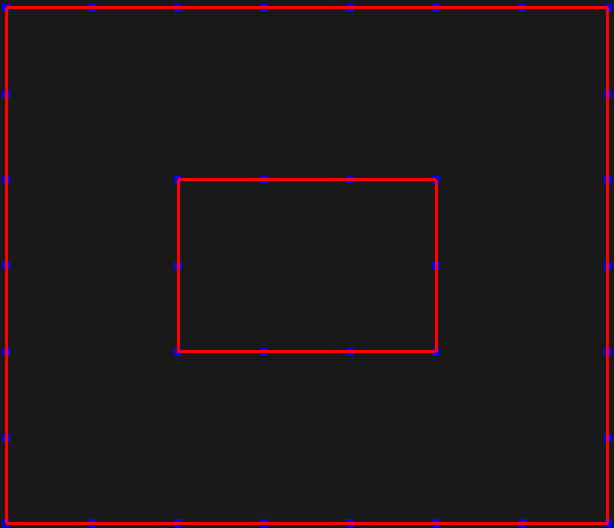
\includegraphics[width = 0.30\textwidth]{front_0.png} & 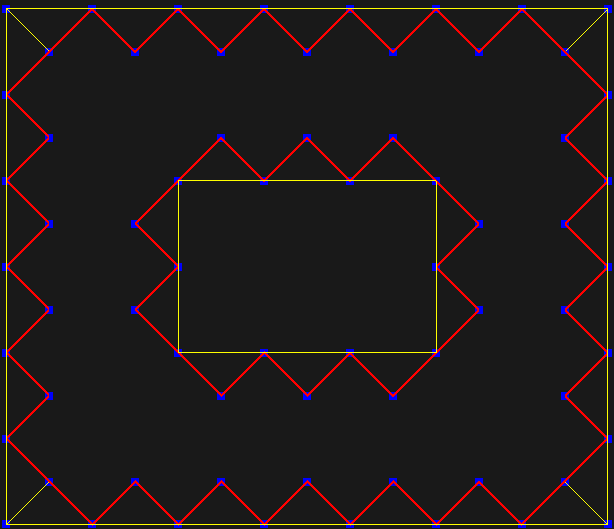
\includegraphics[width = 0.30\textwidth]{front_1a.png} & 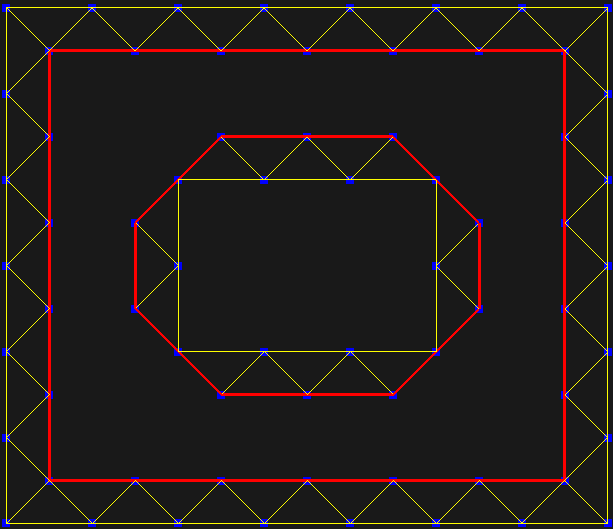
\includegraphics[width = 0.30\textwidth]{front_2a.png} \\
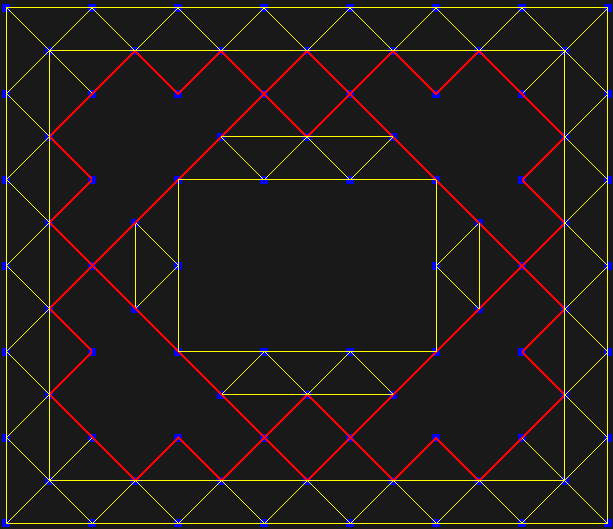
\includegraphics[width = 0.30\textwidth]{front_3a.png} & 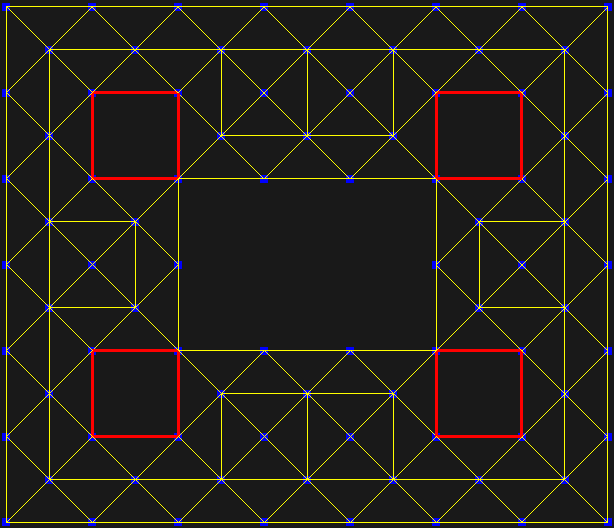
\includegraphics[width = 0.30\textwidth]{front_4a.png} &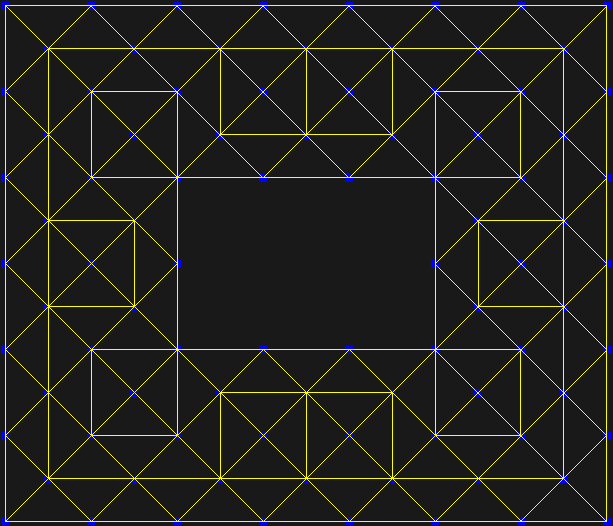
\includegraphics[width = 0.30\textwidth]{front_5a.png} \\
\end{tabular}
\caption{Uniform grid  with active front (red) at different stages during grid generation.}
\label{fig_grida}
\end{center}
\end{figure}

%%%%%%%%%%%%%%%%%%%%%%%%%%%%%%%%%%% fig. 2 %%%%%%%%%%%%%%%%%%%%%%%%%%%%%%%%%%%  
\begin{figure}[htbp] 
\begin{center}
\begin{tabular}{ccc}
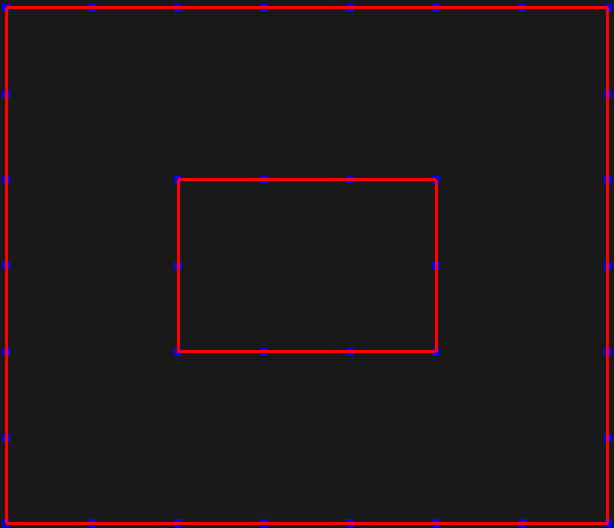
\includegraphics[width = 0.30\textwidth]{front_0.png} & 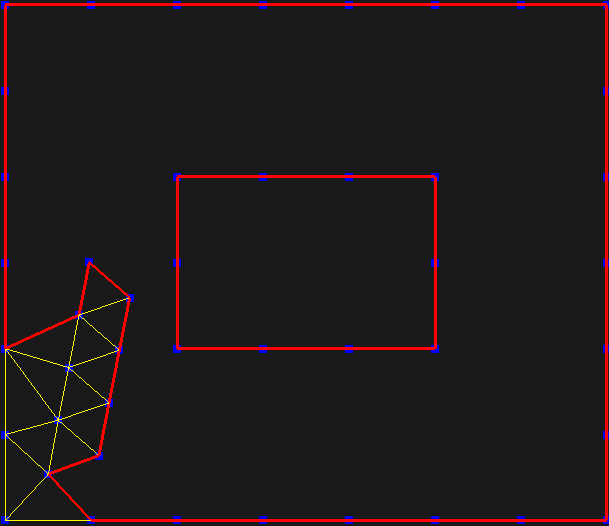
\includegraphics[width = 0.30\textwidth]{front_1b.png} & 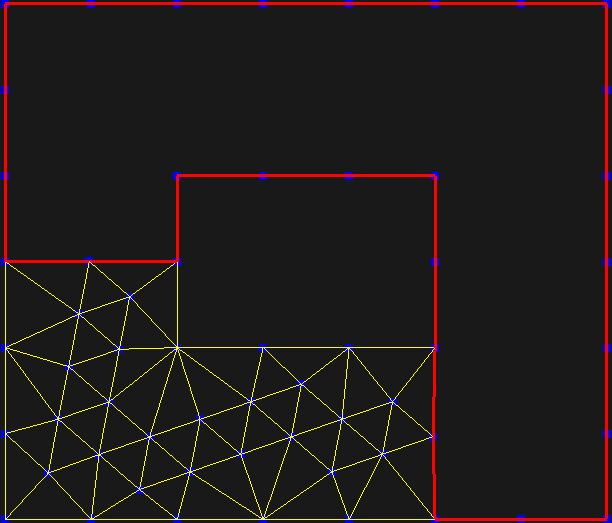
\includegraphics[width = 0.30\textwidth]{front_2b.png} \\
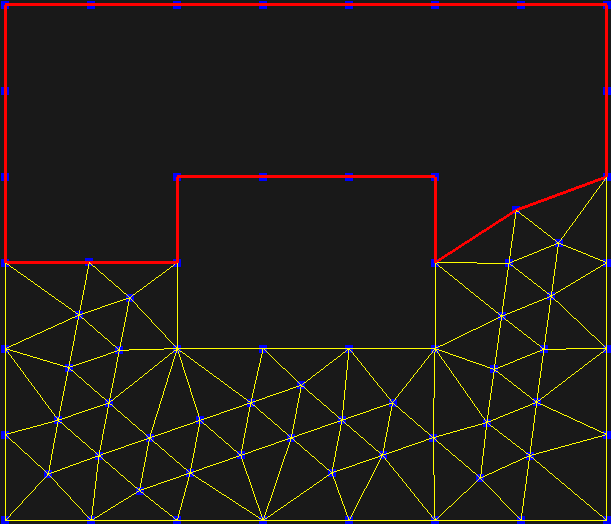
\includegraphics[width = 0.30\textwidth]{front_3b.png} & 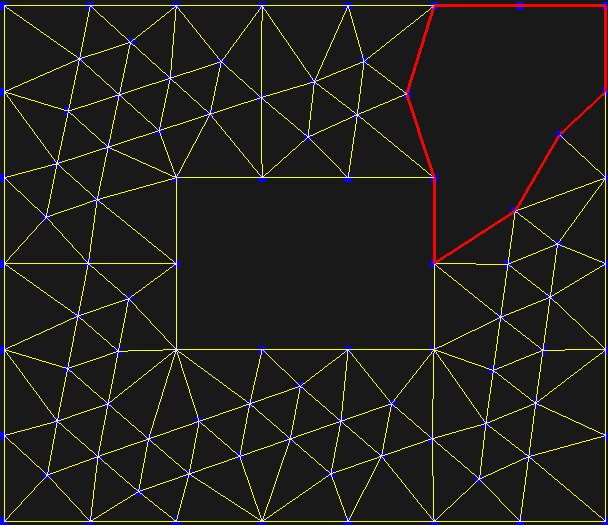
\includegraphics[width = 0.30\textwidth]{front_4b.png} &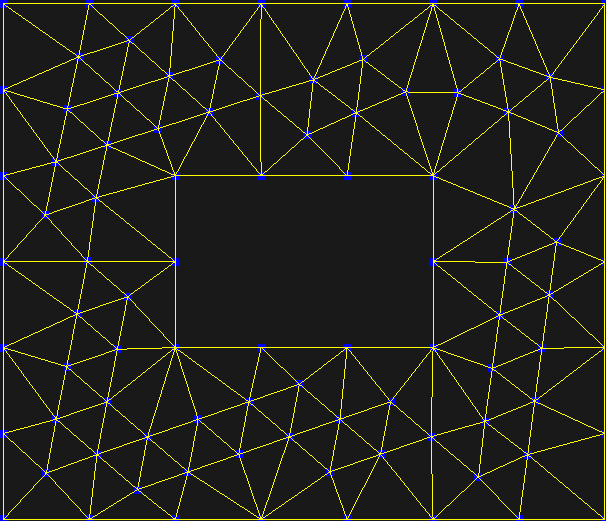
\includegraphics[width = 0.30\textwidth]{front_5b.png} \\
\end{tabular}
\caption{Nonuniform grid  with active front (red) at different stages during grid generation.}
\label{fig_gridb}
\end{center}
\end{figure}


\pagebreak
%%%%%%%%%%%%%%%%%%%%%%%%%%%%%%%%%% Appendix %%%%%%%%%%%%%%%%%%%%%%%%%%%%%%%%%%  
\appendix
\appendixpage

\section{README}\label{app_readme}
The program is mostly automated, but the user must make one small edit to the file 'csi722\_typeDef.f90' to change from uniform to nonuniform grid generation.  To generate a grid of nonuniform elements, open 'csi722\_typeDef.f90'; change the value of the first parameter named 'gtype' from  '0' to '1'.  The programs associated with this project are the following:
\beenum
\item Makefile : Used to compile and execute code.
\item csi722\_project2.f90 : Main program for advancing front algorithm.
\item csi722\_advFront.f90 : External module containing the following subroutines.
\beenum
\item unitNormal : Calculates face normals.
\item updateFaces : Adds/deletes face. Creates new element.
\item intersectTest : Checks if new face intersects any existing faces.
\item getInitGrid : Initial grid is defined.
\item printFaces : Prints current faces to standard output.
\item printElements : Prints current elements to standard output.
\ebenum
\item csi722\_typeDef.f90 : External module containing global parameters and type definitions associated with advancing front algorithm. 
\item csi722\_gridVisual.c : Main program and functions for visualization.
\item faces.h : C header file containing structure definition.
\ebenum

\noindent The advancing front algorithm is compiled and executed with the following terminal command:
\begin{verbatim}
    $ make
\end{verbatim}
The visualization is compiled and executed with the following terminal command:
\begin{verbatim}
    $ make visual
\end{verbatim}
All modules, object files and executables are removed with the following terminal command:
\begin{verbatim}
    $ make clean
\end{verbatim}

%% \bibliographystyle{plain}	% (uses file "plain.bst")
%% \bibliography{myrefs}		% expects file "myrefs.bib"

\end{document}
